\begin{frame}{Akash idea for future work}
	\begin{itemize}
		\item Since flip-flops contain lot of useful information than just the state (for e.g:., information about future instructions, branching etc.), is it possible to lock sequential circuits in a different way ? For e.g:., encrypting Processor FSM in some new meaningful way ?
		\item The encryption should not just be similar to adding few gates on flip-flops, rather some complex encryption scheme that considers the instructions, data flow, FSM etc. 
	\end{itemize}
\end{frame}

\begin{frame}{Akash feedback}
\begin{itemize}
\item How does the decryption runtime change if systematically one-by-one the key gates are removed from the combinational logic ? If runtime does not reduce drastically, then there is huge area savings (because 50\% of the circuit is encrypted) 
\item Agreed that the SAT solver returned different key for sequential locked case for c880
	\begin{itemize}
	\item Will the different key also activate the IC, for correct functional operation ?
	\item Is there a case (any of the benchmarks), where the SAT solver is returning the correct key ?
	\item Can we come up with a heuristic, which ensures the solver comes up with a key that will produce wrong functional operation ?
	\end{itemize}
\item Use GIT to write the paper (both .docx and latex).
\end{itemize}
\end{frame}

\begin{frame}{Proposed Experiments}
	\begin{itemize}
		\item Since SAT-attack tool deals with bench format, try ITC'99 circuits because they are already available in bench format\footnote{http://www.pld.ttu.ee/~maksim/benchmarks/}
		\item Remove flip-flops and create pseudo-primary-inputs/outputs, and create original-type bench files
		\item Add combinational-logic-locking gates and create combinational-encrypted-type bench files
		\item On top of this, add sequential-locking-unrolling gates and create sequential-combinational-encrypted-type bench files
		\item Before implementing proposed technique on ITC'99 circuits, first check if SAT-attack is successful on large ITC'99 circuits - \alert{checking if SAT-attack is scalable}
	\end{itemize}
\end{frame}

\begin{frame}{Some results}
	\begin{itemize}
		\item \texttt{b18, b19}, encryption with \alert{only 1 key-bit}
%		\item As of 9:30 am CET on September 7, 2018 the run is still in progress (\alert{$\approx$ 44 hours})
		\item The run took 91m 3s, and 256m 57s, respectively to decrypt the 1-key bit. 
		\item I think this is the reason, researchers working on logic locking, partition the circuit and launch the SAT-attack on the individual partitions. 
		\item But I don't see the point in partitioning and then do SAT-solving on individual partitions, because the SAT solver should do the same thing anyway. 
	\end{itemize}
\end{frame}

\begin{frame}{Some more important observations}
	\begin{itemize}
		\item Combinational logic locking is vulnerable to removal attack
		\item Sequential logic locking is \alert{NOT} vulnerable to removal attack
		\item Limitations on {\it Encrypt Flip-Flop} paper from IIT-KGP. 
			\begin{itemize}
				\item Adding XOR gates into netlist increases physical design effort
				\item Partitioning the circuit, and attacking individual partitions is not possible, because the outputs of some partitions are {\it internal nodes}, whose logic states are not known (only the states of primary inputs and primary outputs are known in SAT-based attack)
			\end{itemize}
	\end{itemize}
\end{frame}

\begin{frame}{Some more important observations}
	\begin{itemize}
		\item \texttt{b03}: if encrypting only scan-chain, and no logic-locking, key is getting decrypted in 1.45s
		\item San-unrolled circuit for \texttt{b03}, is as big as scan-unrolled circuit for \texttt{c880} (with scan-cells at primary outputs), however in latter case, it took more than 100s
		\item Conclusion: if only locking flip-flops, it gets decrypted very fast, because it is only XOR chain, which is easy to decode
		\item However, next and more important question is about correctness of the decrypted key ?
	\end{itemize}
\end{frame}

\begin{frame}{Verification with \texttt{c880}}
	\begin{figure}
		\begin{center}
		\label{fig:c880-c-l}
		\caption{Combinational locking; Solver Key $\{\alert{k_{18}, k_{97}, k_{111}, k_{133}}\} = \{\alert{1,1,0,1}\}$}
			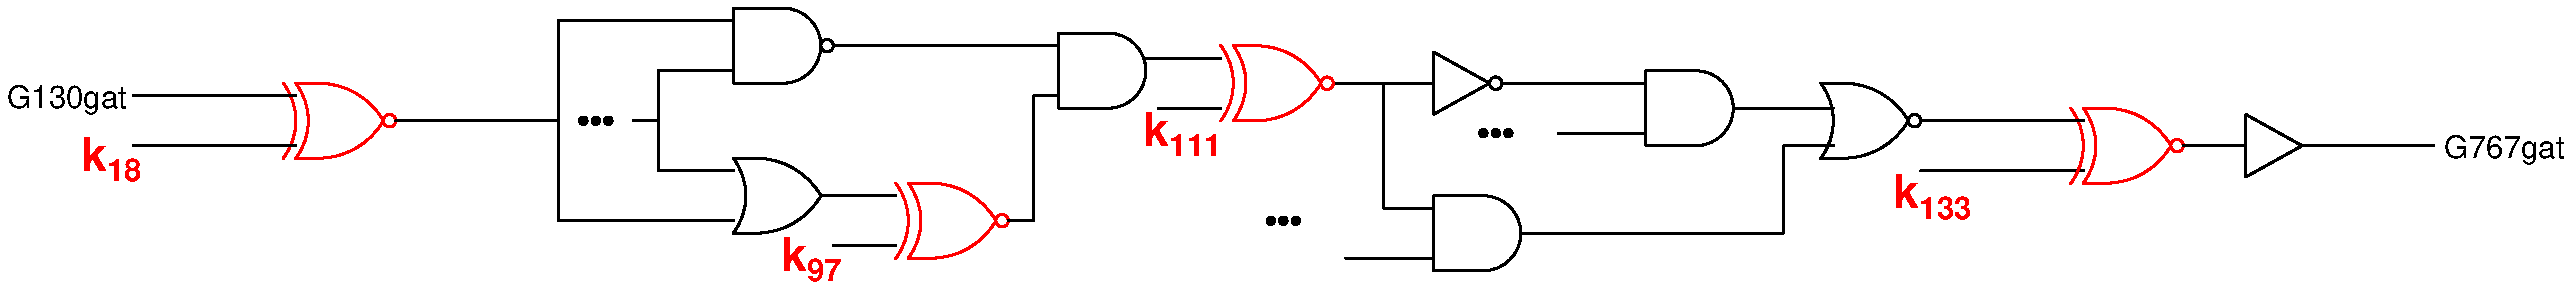
\includegraphics[scale=0.2]{fig/c880_combinational_locking_motivation.pdf}
		\end{center}
	\end{figure}
	\begin{figure}
		\begin{center}
		\label{fig:c880-s-c-l}
		\caption{Sequential locking; Solver Key $\{\alert{k_{18}, k_{97}, k_{111}, k_{133}}, k_{207}, k_{206}, k_{205}, \ldots k_{192}\} = \{\alert{0,1,1,0},0,0,0,1,0,0,1,0,0,0,0,1,0,0,0,0\}$}
			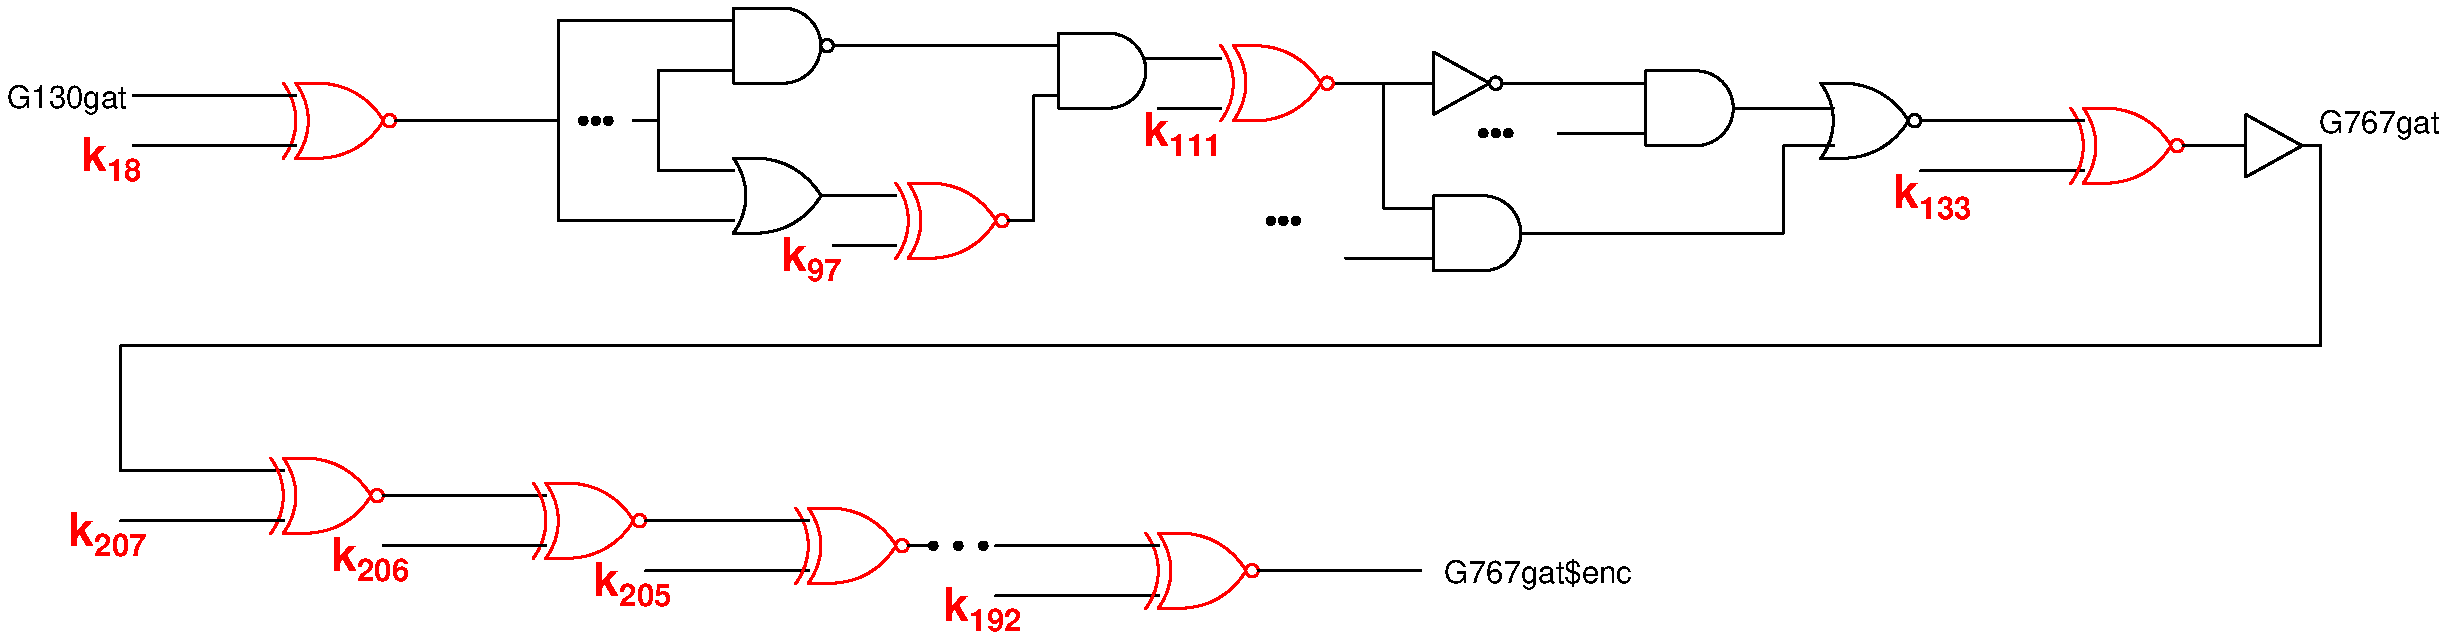
\includegraphics[scale=0.2]{fig/c880_sequential_combinational_locking_motivation.pdf}
		\end{center}
	\end{figure}
\end{frame}

\begin{frame}{Verification with \texttt{c880}}
\begin{itemize}
\item \texttt{c880} with combinational locking: key is \alert{1101}, which is odd-inversion-parity
\item \texttt{c880} with sequential locking: combinational portion of the key is \alert{0110}, which is even-inversion-parity
\item Thus, for chip that uses sequential locking, during functional mode of operation, the signal undergoes \alert{wrong} number of inversions before it reaches the destination flip-flop, thus corrupting the circuit state.
\item When the SAT-attack decrypted key is applied: during scan, the circuit functions correctly, but during functional mode of operation, it is corrupt. 
\end{itemize}
\end{frame}
